%%%%%%%%%%%%%%%%%%%%%%%%%%%%%%%%%%%%%%%%%
% Short Sectioned Assignment LaTeX Template Version 1.0 (5/5/12)
% This template has been downloaded from: http://www.LaTeXTemplates.com
% Original author:  Frits Wenneker (http://www.howtotex.com)
% License: CC BY-NC-SA 3.0 (http://creativecommons.org/licenses/by-nc-sa/3.0/)
%%%%%%%%%%%%%%%%%%%%%%%%%%%%%%%%%%%%%%%%%

% \documentclass[paper=a4, fontsize=11pt]{scrartcl} % A4 paper and 11pt font size
\documentclass[11pt, a4paper]{book}
\usepackage[T1]{fontenc} % Use 8-bit encoding that has 256 glyphs
\usepackage[utf8]{inputenc}
\usepackage{fourier} % Use the Adobe Utopia font for the document - comment this line to return to the LaTeX default
\usepackage{listings} % para insertar código con formato similar al editor
\usepackage[spanish, es-tabla]{babel} % Selecciona el español para palabras introducidas automáticamente, p.ej. "septiembre" en la fecha y especifica que se use la palabra Tabla en vez de Cuadro
\usepackage{url} % ,href} %para incluir URLs e hipervínculos dentro del texto (aunque hay que instalar href)
\usepackage{graphics,graphicx, float} %para incluir imágenes y colocarlas
\usepackage[gen]{eurosym} %para incluir el símbolo del euro
\usepackage{cite} %para incluir citas del archivo <nombre>.bib
\usepackage{enumerate}
\usepackage{hyperref}
\usepackage{graphicx}
\usepackage{tabularx}
\usepackage{booktabs}

\usepackage[table,xcdraw]{xcolor}
\hypersetup{
	colorlinks=true,	% false: boxed links; true: colored links
	linkcolor=black,	% color of internal links
	urlcolor=cyan		% color of external links
}
\renewcommand{\familydefault}{\sfdefault}
\usepackage{fancyhdr} % Custom headers and footers
\pagestyle{fancyplain} % Makes all pages in the document conform to the custom headers and footers
\fancyhead[L]{} % Empty left header
\fancyhead[C]{} % Empty center header
\fancyhead[R]{Moisés Téllez Francisco} % My name
\fancyfoot[L]{} % Empty left footer
\fancyfoot[C]{} % Empty center footer
\fancyfoot[R]{\thepage} % Page numbering for right footer
%\renewcommand{\headrulewidth}{0pt} % Remove header underlines
\renewcommand{\footrulewidth}{0pt} % Remove footer underlines
\setlength{\headheight}{13.6pt} % Customize the height of the header

\usepackage{titlesec, blindtext, color}
\definecolor{gray75}{gray}{0.75}
\newcommand{\hsp}{\hspace{20pt}}
\titleformat{\chapter}[hang]{\Huge\bfseries}{\thechapter\hsp\textcolor{gray75}{|}\hsp}{0pt}{\Huge\bfseries}
\setcounter{secnumdepth}{4}
\usepackage[Lenny]{fncychap}


\begin{document}

	% Plantilla portada UGR
	\begin{titlepage}
\newlength{\centeroffset}
\setlength{\centeroffset}{-0.5\oddsidemargin}
\addtolength{\centeroffset}{0.5\evensidemargin}
\thispagestyle{empty}

\noindent\hspace*{\centeroffset}\begin{minipage}{\textwidth}

\centering

\includegraphics[width=0.9\textwidth]{logos/logo_ugr.jpg}\\[1.4cm]

\textsc{ \Large TRABAJO FIN DE GRADO\\[0.2cm]}
\textsc{ GRADO EN INGENIERIA INFORMATICA}\\[1cm]

{\Huge\bfseries Generador de esculturas
abstractas a partir de
modelos 3D\\}
\noindent\rule[-1ex]{\textwidth}{3.5pt}\\[3.5ex]
{\large\bfseries Subtítulo }
\end{minipage}

\vspace{2.5cm}
\noindent\hspace*{\centeroffset}
\begin{minipage}{\textwidth}
\centering

\textbf{Autor}\\ {Moisés Téllez Francisco}\\[2.5ex]
\textbf{Director}\\ {Francisco Javier Melero Rus}\\[2cm]

\includegraphics[width=0.3\textwidth]{logos/etsiit_logo.png}\\[0.1cm]
\textsc{Escuela Técnica Superior de Ingenierías Informática y de Telecomunicación}\\
\textsc{---}\\
Granada, Junio de 2023
\end{minipage}
\end{titlepage}


	% Plantilla prefacio UGR
	\thispagestyle{empty}

\begin{center}
{\large\bfseries Generador de esculturas
abstractas a partir de
modelos 3D }\\
\end{center}
\begin{center}
Moisés Téllez Francisco\\
\end{center}

%\vspace{0.7cm}

\vspace{0.5cm}
\noindent\textbf{Palabras clave}: \textit{software libre, Graficos por ordenador, Shaders, Pablo Gargallo, Modelos 3D, Esculturas, Arte Abstracto, OpenGL}
\vspace{0.7cm}

\noindent\textbf{Resumen}\\

El objetivo de este trabajo es abordar la generación automática de esculturas abstractas a traves de software. Este problema es extenso
y puede ser abordado desde muchos ambitos, en este caso nos hemos centrado en imitar el estilo de un solo escultor, Pablo Gargallo, que en sus obras utilizaba
la relacion entre las concavidades y las convexidades para lograr volumenes que no son posibles de obtener utilizando las tecnicas convencionales. Nuestro objetivo final
es conseguir un software que genere una version ``Gargallesca`' de cualquier escultura correctamente digitalizada a partir del punto de vista del observador
	

\cleardoublepage

\begin{center}
	{\large\bfseries Abstract Sculpture generation from 3D Models}\\
\end{center}
\begin{center}
	Moisés Téllez Francisco\\
\end{center}
\vspace{0.5cm}
\noindent\textbf{Keywords}: \textit{open source, Computer graphics, Shaders, Pablo Gargallo, 3D Models, Sculptures, Abstract Art, OpenGL}, \textit{floss}
\vspace{0.7cm}

\noindent\textbf{Abstract}\\


\cleardoublepage

\thispagestyle{empty}

\noindent\rule[-1ex]{\textwidth}{2pt}\\[4.5ex]

D. \textbf{Francisco Javier Melero Rus}, Profesor del ...

\vspace{0.5cm}

\textbf{Informo:}

\vspace{0.5cm}

Que el presente trabajo, titulado \textit{\textbf{Chief}},
ha sido realizado bajo mi supervisión por \textbf{Estudiante}, y autorizo la defensa de dicho trabajo ante el tribunal
que corresponda.

\vspace{0.5cm}

Y para que conste, expiden y firman el presente informe en Granada a Junio de 2018.

\vspace{1cm}

\textbf{El/la director(a)/es: }

\vspace{5cm}

\noindent \textbf{Francisco Javier Melero Rus}

\chapter*{Agradecimientos}






	% Índice de contenidos
	\newpage
	\tableofcontents

	% Índice de imágenes y tablas
	\newpage
	\listoffigures

	% Si hay suficientes se incluirá dicho índice
	\listoftables 
	\newpage

	% Introducción 
	\chapter{Introducción}

\section{Introducción}
El objetivo de este proyecto es la creación de un software capaz de transformar de forma autonoma un modelo 3D detallado de una escultura cualquiera en una escultura que inmita el estilo del escultor Pablo Emilio Gargallo Catalán.
Este estilo se caracteriza principalmente por jugar con las concavidades y las convexidades de las esculturas para obtener efectos no obtenibles por medio de tecnicas tradicionales.

\begin{figure}
    \centering
    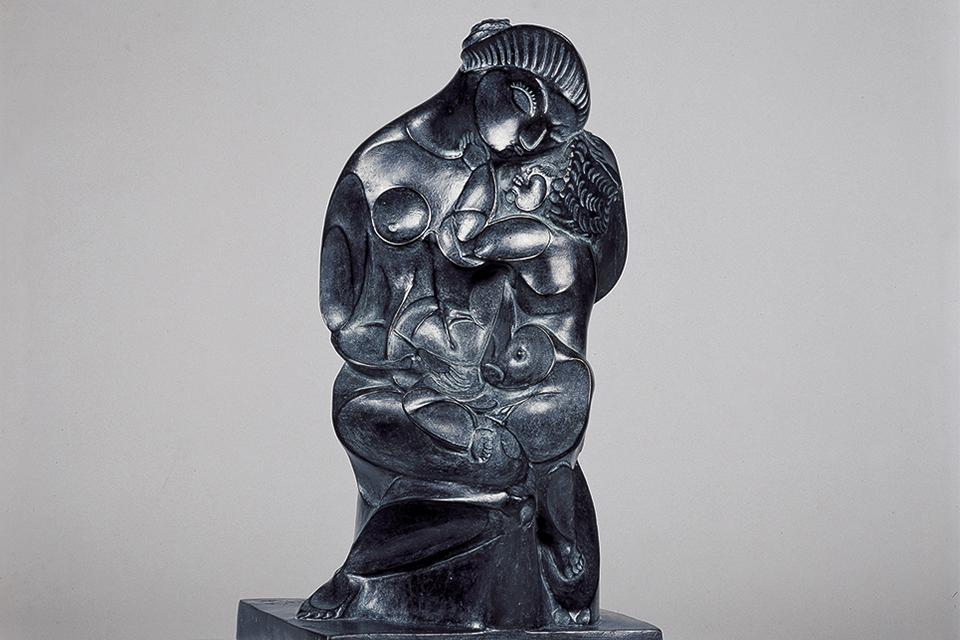
\includegraphics[width=\textwidth]{imagenes/maternidad_gargallo.jpg}
    \caption{Ejemplo de una escultura de Pablo Gargallo}
\end{figure}


Nuestro punto focal de interes va a ser precisamente lograr transformar las convexidades de los modelos 3D en concavidades. Para permitirnos hacer esto vamos a utilizar varios recursos de los graficos por ordenador.

El termino graficos por ordenador se refiere a un campo multidisciplinar donde se agrupa cualquier disciplina que contribuye a la creación y visualización de representaciones pictoricas enteremante en un ordenador\cite{Foley_1995}.
Esto engloba una variedad de campos donde hay discusión sobre si pertenecen o no al ambito de los graficos por ordenador.Sin embargo hay 3 campos principales en los cuales hay consenso general de que forman parte de la disciplina.
\begin{list}{.}{}
    \item El modelado, que es la rama que lidia con la representación matematica de la especificación de la forma y la apariencia de una representación pictorica concreta de forma que sea interpetable para un ordenador
    \item El Renderizado, que lidia con la creación de las representaciones 2D finales de nuestros modelos 3D tras la aplicación de luces, texturas y materiales 
    \item La animación que es la tecnica para crear ilusión de movimiento a partir de la secuenciación de Imagenes. Dentro de esta rama se utilizan conceptos del renderizado y el modelado pero se le añade el factor clave del movimiento en el tiempo
\end{list} \cite{marschner_fundamentals_2018}

Para nuestro proyecto los campos relevantes son solo el modelado y el renderizado. Puesto que al final del proyecto nuestro objetivo es poder visualizar de forma dinamica esa escultura "Gargallizada" y ademas poder exportar una representación de la escultura luego de ser modificada para poder ser impresa en 3D.

La capacidad de poder visualizar los graficos por ordenador necesitamos generar una imagen sintetica en dos dimensiones que pueda ser representada sobre la pantalla del ordenador. Para ello se definen todos los elementos del entorno tridimensional, siendo esto no solo los modelos tridimensionales sino tambien la presencia de luces. Las cuales de hecho son obligatorias. Pues sin ellas todo se vería oscuro. 
En su defecto las API de graficos por ordenador utilizan una luz ambiente que aplica de igual forma a todos los elementos. Y finalmente el ultimo elemento necesario es una camara que nos permite crear un sentido de perspectiva y colocar un punto de referencia desde el cual se esta visualizando la escena.

Una vez todos los elementos estan definidos la API de graficos que vayamos a utilizar realizara una serie de operaciones para conseguir esa representacion pictorica bidimensional de nuestro modelo. Esta serie de operaciones es lo que conocemos como "pipeline" de graficos. De forma simple esta serie de operaciones son fijas y para cualquier modelo seran siempre las mismas. Este pipeline de transformaciones dependera del proceso que utilice la API de graficos para generar
la imagen bidimensional final. En  nuestro caso para este trabajo estamos utilizando OpenGL, la cual es una API de graficos que utiliza rasterización para el renderizado. Pero existen otras alternativas que recientemente estan cobrando mas popularidad como el Ray Tracing. Como hemos mencionado previamente en este trabajo hemos decidido emplear OpenGL como API de graficos. Esto se debe principalmente a dos motivos. El primero es uno de familiaridad puesto que OpenGL es la API de graficos
que se enseña en el grado. Ademas de eso el segundo motivo es que OpenGL es la API mas extendida entre todas las alternatives libres y multiplatadorma. Y aunque tiene competidores directos como la API Direct3D estos son privativos. Cabe mencionar que existe un estandar alternativo a OpenGL mas moderno llamado Vulkan, el cual permite un mayor control sobre lo que ocurre en la tarjeta grafica y ofrece un mayor rendimiento. Sin embargo el punto donde las diferencias de rendimiento entre Vulkan y OpenGL 
se hace notable es en proyectos mucho mas ambiciosos como videojuegos triple A con graficos hiperrealistas. Para nuestro proyecto elegir una u otra es indiferente. Y por tanto decidimos utilizar la API que ya conociamos y teniamos cierta experiencia previa.

Explicación Pipeline fija de graficos

Explicación Pipeline programable de graficos

Detección de profundidades

\begin{figure}
    \centering
    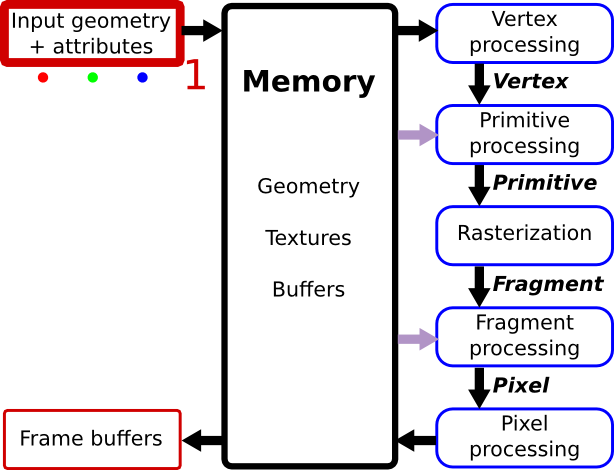
\includegraphics[width=\textwidth]{imagenes/Pipeline_Fija.png}
    \caption{Pipeline de graficos fija de OpenGL}
    \cite{freeSI03graphicsPipeline}
\end{figure}

En este caso el pipeline de graficos se compone 

\section{Motivación}

Este proyecto es software libre, y está liberado con la licencia \cite{gplv3}.



	% Descripción del problema y hasta donde se llega
	\chapter{Descripción del problema}



	% Estado del arte
	% 	1. Crítica al estado del arte
	% 	2. Propuesta
	\chapter{Estado del arte}

El software libre y sus licencias \cite{gplv3} ha permitido llevar a cabo una expansión del
aprendizaje de la informática sin precedentes.

	
	\chapter{Planificación}

\section{Metodología utilizada}


\section{Temporización}

\section{Seguimiento del desarrollo}


	% Análisis del problema
	% 1. Análisis de requisitos
	% 2. Análisis de las soluciones
	% 3. Solucion propuesta
	% 4. Análisis de seguridad
	\chapter{Análisis del problema}
 


	% Desarrollo bajo sprints: 
	% 	1. Permitir registros y login de usuarios
	% 	2. Desarrollo del sistema de incidencias
	% 	3. Desarrollo del sistema de denuncias administrativas y accidentes
	% 	4. Desarrollo del sistema de croquis
	%   5. Instalación de la aplicación de manera automática
	\chapter{Implementación}

La implementación del software se ha dividido en hitos. Estos, han sido definidos en Github
y cada uno de ellos contiene un grupo de \textit{issues} que se corresponden con las distintas
mejoras que se han ido incorporando al software a lo largo de su desarrollo.\\



	% Presupuesto

	% Conclusiones
	\chapter{Conclusiones y trabajos futuros}



	% Trabajos futuros


	
	\newpage
	\bibliography{bibliografia}
	\bibliographystyle{plain}
	
\end{document}

